\section{Overview of \name}
\label{sec:overview}

To optimize inter-DC multicasts while minimizing
interference with latency-sensitive traffic, we present {\em \name},
a near-optimal inter-DC multicast overlay network.
%Unlike previous designs where individual servers always retain
%some local control capability,
%\name {} {\em fully centralizes} the
%control of the multicast overlay network.
Before presenting \name in details,
we first highlight the intuitions behind its
key design choice, and the challenges to make it practical.


%\name is built on a couple of design choices, which
%trade marginal costs for substantial performance benefits.
%Before describing the details of \name's design, we first
%highlight the design choices and the intuition behind
%their cost-benefit tradeoffs
%(summarized in Table~\ref{tab:design-choices}).



%The insights obtained from \company's operational experience has inspired the design of \name, a near-optimal inter-DC multicast overlay network. This section starts with \name key design choices, highlights the design philosophy behind our choices, and provide an overview of the \name system, which builds on these design choices.

%\subsection{Why a fully centralized design}

\mypara{Centralized control}
Conventional wisdom on wide-area overlay networks
always rely on local adaptation of individual
nodes to achieve desirable scalability
and responsiveness to network dynamics (e.g.,~\cite{Andreev2013Designing,Repantis2010Scaling,Huang2014A}),
despising the suboptimal performance due to
the lack of global view and coordination.
Recent work (e.g.,~\cite{mukerjee2014enabling}), however,
shows the feasibility of combining real-time
local adaptation with a centralized logic operating
on coarser timescales.
In contrast, \name takes an explicit stance that
fully centralized control is practical,
and shows that it can achieve near-optimal performance in
the setting of inter-DC multicasts.
%, near-optimal performance can be achieved through a fully centralized design.
As illustrated in Figure~\ref{fig:framework},
\name uses a centralized controller that periodically pulls
information from all servers, updates the decisions regarding overlay
routing, and pushes them to agents running locally on servers.
Note that when the controller fails or is unreachable,
\name will fall back to a decentralized scheme
to ensure graceful performance degradation.

%Stemming from suboptimal local adaptation decisions made by individual servers in lack of global view and coordination, many prior approaches~\cite{Andreev2013Designing,Repantis2010Scaling,Huang2014A}, including \company's system suffer from the limitations highlighted in \Section\ref{subsec:motivation:baseline}. These limitations remain in hybrid control schemes (e.g.,~\cite{yin2009design,mukerjee2014enabling}) which combines real-time local adaptation with a centralized logic operating on coarser timescales. In other words, the conventional wisdom prefer local adaptation for desirable scalability and responsiveness, thus unavoidably resulting in performance suboptimality.

\begin{figure}[t]
  \centering
  %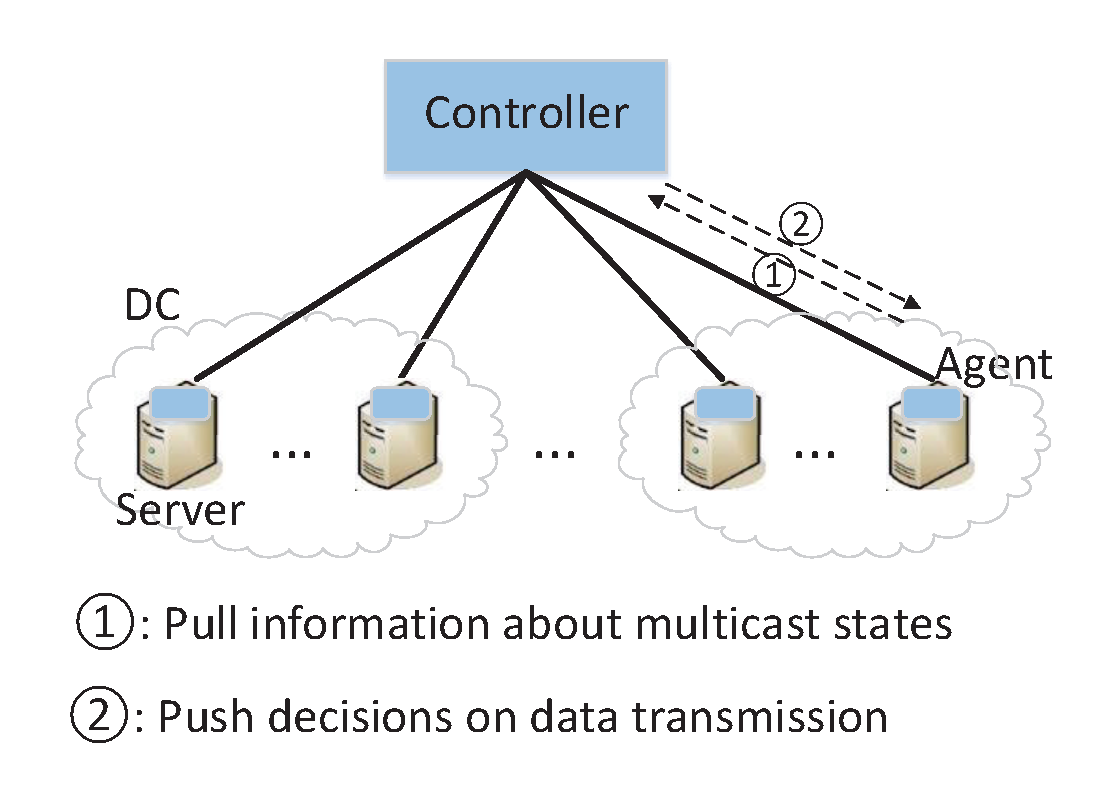
\includegraphics[width=2in]{images/framework.eps}
  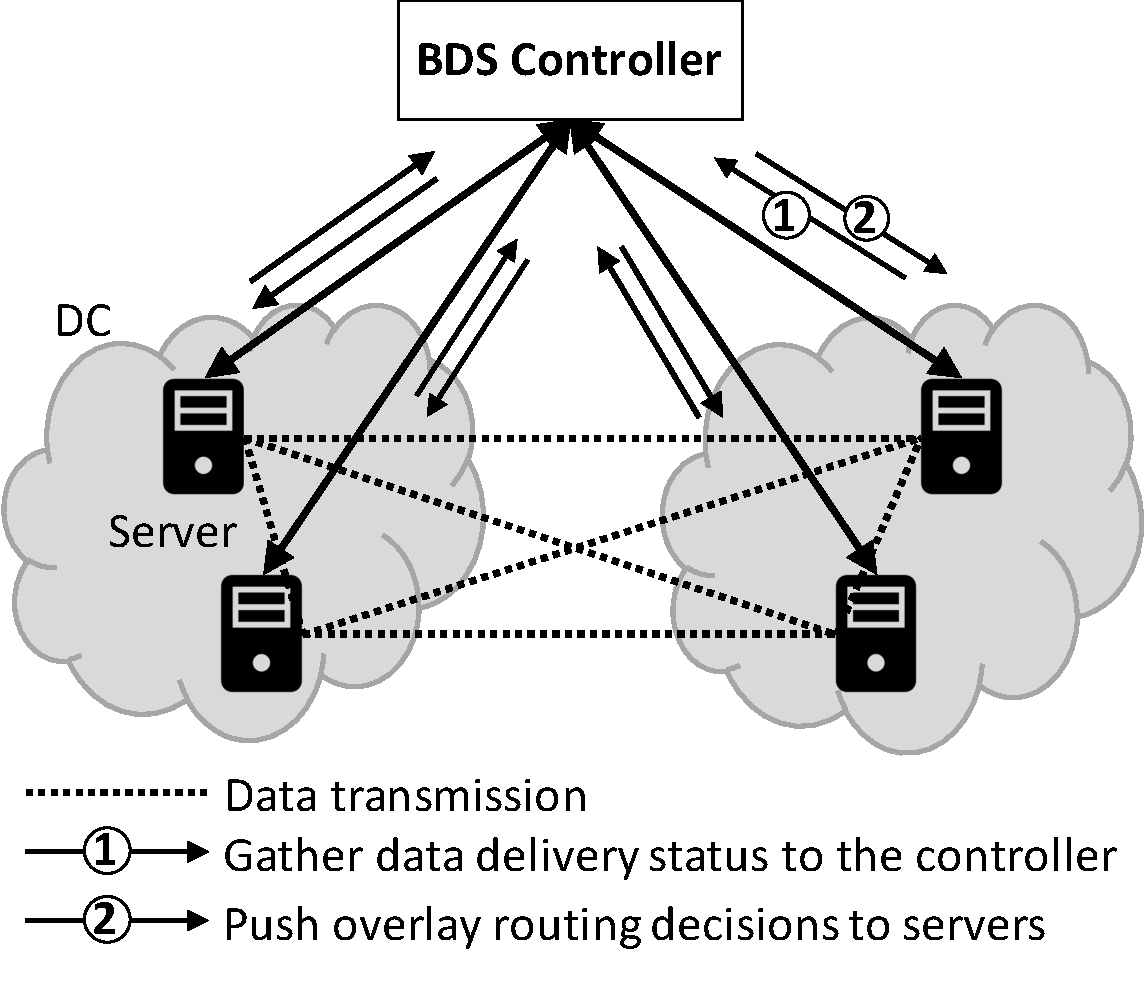
\includegraphics[width=2.3in]{images/framework-new.pdf}
  \tightcaption{The centralized design of \name.}
  \label{fig:framework}
\vspace{-0.4cm}
\end{figure}

%\mypara{Centralized design}
%Specifically, the controller schedules data transfers, make the path selection and bandwidth allocation for each transfer in each scheduling period.
%\mypara{Design philosophy}

Our centralized design is driven by four considerations:
\begin{packedenumerate}

\item {\em Large decision space:}
The sheer numbers of inter-DC overlay paths,
which grow exponentially with more servers acting as overlay nodes,
make it hard for servers to explore all possible overlay
paths based only on local measurements.
Instead, we could significantly improve overlay multicast
performance by maintaining a global view of data delivery
status of all servers and dynamically balance
the availability of
various data blocks, which
is critical to achieving near-optimal performance
(\Section\ref{subsec:logic:scheduling}).

\item {\em Large data size:}
Unlike latency-sensitive traffic
(e.g., online partition and aggregation) which lasts on timescales
of 10s to 100s of milliseconds, inter-DC multicasts are large in volume and
last on a much coarser timescale.
Thus, being highly responsive to transient network dynamics is a necessary concern.
%In this context, the tradeoff between a centralized design and a decentralized one is that centralized control essentially trades real-time responsiveness to network dynamics for closer-to-optimal control decisions driven by a global view of data delivery. Here,
\name tolerates a short delay (of a few seconds) to query a centralized controller
which could make closer-to-optimal decisions based on a global view of data delivery.

\item {\em Strict traffic isolation:}
As observed in \Section\ref{subsec:motivation:baseline},
it is vital that inter-DC
multicasts avoid hotspots and excessive bandwidth usage that can increase the latency of delay-sensitive traffic,
but it is difficult to prevent such situations
without any coordinations across overlay servers.
In contrast, it is practical
to determine the bandwidth allocation and periodically update it
to all servers in a centralized fashion (\Section\ref{sec:system}).

\item {\em Simple engineering:}
Conceptually, the centralized architecture moves the complexity to
the centralized controller, making \name amenable to a simple implementation,
where the control logic running locally in each server can be stateless and
triggered only on arrivals of new data units or control messages.

\end{packedenumerate}

%\mypara{Fast and near-optimal decision-making}
\mypara{The key to realizing centralized control}
In essence, \name trades updating decisions on coarse timescales
for the potential of making optimal decisions in a centralized
fashion.
The key to striking such a favorable balance is a
near-optimal and efficient overlay routing
algorithm that can be updated on near-realtime timescales.
At a first glance, this is indeed intractable:
the centralized overlay routing algorithm must pick the next hops
from $10^4$s of servers for $10^5$s of blocks, a scale that could
grow exponentially when we consider all possible
overlay paths that go through these servers and more fine-grained block partitions.
%It is unclear how this problem can be solved even with limited approximation, which was partly why \company has been lukewarm about a centralized control architecture, despite its potential benefits.
The next section will present how \name addresses this challenge.

%The key technical challenge here is how to make optimal overlay scheduling and routing decisions at the scale tens of thousands of objects and tens of thousands of servers in near real time. To achieve desirable performance in a multicast overlay network, fully exploiting all the available overlay paths is essential, but it is untenable to go through all the potential servers and exponentially more paths by traditional approaches.

%\begin{itemize}
%
%\item Idea \#1: Fully centralized control
%
%\item Idea \#2: Dynamic bandwidth separation: separating background bulk data transfer from latency-sensitive traffic
%
%\item These ideas introduces performance costs (not real time, potentially low link utilization) are outweighed by benefits (not real time, potentially low link utilization)
%
%\item Design philosophy: the costs are outweighed by the benefits. (1) bulk data transfer can tolerate updates at coarse timescales. (2) the aggregation of latency-sensitive data is stable on timescales of several seconds. (3) the resulting system is amenable to simpler implementation.
%
%\item Key technical challenge: how to make optimal overlay scheduling and routing decisions at the scale tens of thousands of objects and tens of thousands of servers in near real time.
%
%\end{itemize}



